\setlength{\columnsep}{3pt}
\begin{flushleft}
\bigskip
Step 5: Stage 1 bootloader

\begin{itemize}
	\item This first 512 bytes of HDD is too small to fit an entire boot loader program to it.
	\item Hence only the stage 1 bootloader program is present in initial 446 bytes of MBR.
	\item This stage 1  bootloader load the stage 2 boot loader \& file system drivers to the RAM.
\end{itemize}

\begin{figure}[h!]
	\centering
	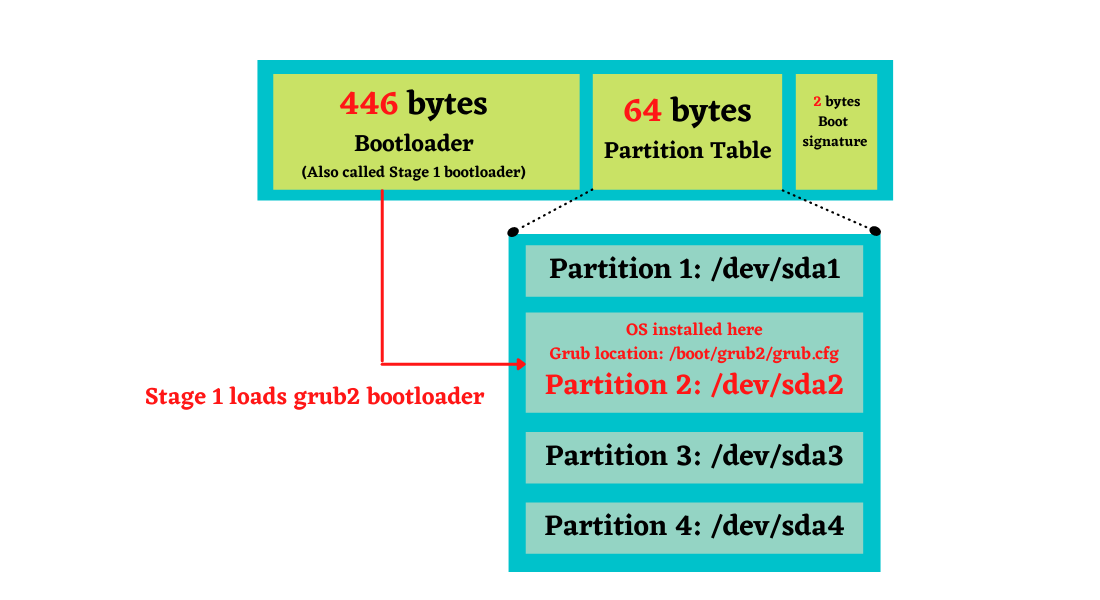
\includegraphics[scale=0.6]{content/chapter17/images/grub2.png}
	\caption{Stage 1 bootloader loading stage 2}
	\label{fig:stage}
\end{figure}

\newpage
Step 6: Stage 2 bootloader also known as \textbf{Grub2}
\begin{itemize}
	\item \textbf{GRUB2 (GRand Unified Boot Loader version 2)} does the job of loading the kernel (Eg: /boot/vmlinuz-4.18.0-348.el8.x86\_64) in RAM.
	\item Grub 2 configuration file: \textbf{/boot/grub/grub.conf}.
	\item At this stage, you are presented with a \textbf{TUI (Terminal user
	interface)}, where you can select your operating system kernel and press enter to boot it.
\end{itemize}
	
\begin{figure}[h!]
	\centering
	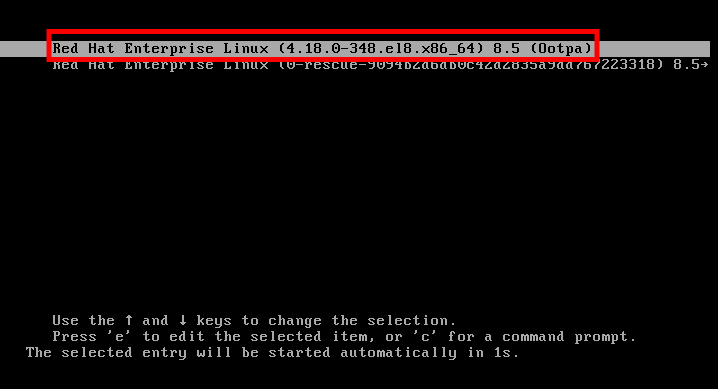
\includegraphics[scale=0.5]{content/chapter17/images/grub_tui.png}
	\caption{TUI}
	\label{fig:stage}
\end{figure}

Step 7: Initrd image also known as \textbf{initramfs}
\begin{itemize}	
	\item The Linux kernel loads initrd (Initial Ramdisk).
	\item The kernel uses initrd image files (Eg: /boot/initramfs-4.18.0-348.el8.x86\_64.img) as a \textbf{temporary virtual filesystem} in the memory.
\end{itemize}

Step 8: Linuxrc file
\begin{itemize}
	\item Next, the linuxrc script is executed that creates temporary device nodes in /dev, waits and mount rootfs, switches to real root.
\end{itemize}
\newpage
Step 9: Kernel stage
\begin{itemize}
	\item The Linux kernel based on the result of linuxrc, mount the real root file system i.e "/".
	\item The \textbf{kernel will then start the init process with process ID "1"} as first background process.
\end{itemize}

Step 10: init/systemd process
\begin{itemize}
	\item On RHEL 8, /sbin/init is link to \textbf{/lib/systemd/systemd}.
	\item \textbf{systemd} looks for \textbf{default target} and starts all the units under it.
\end{itemize}


Let's see more on \textbf{runlevels/target} in Linux.

\end{flushleft}
\newpage


